% Options for packages loaded elsewhere
\PassOptionsToPackage{unicode}{hyperref}
\PassOptionsToPackage{hyphens}{url}
%
\documentclass[
  12pt,
]{article}
\usepackage{lmodern}
\usepackage{amssymb,amsmath}
\usepackage{ifxetex,ifluatex}
\ifnum 0\ifxetex 1\fi\ifluatex 1\fi=0 % if pdftex
  \usepackage[T1]{fontenc}
  \usepackage[utf8]{inputenc}
  \usepackage{textcomp} % provide euro and other symbols
\else % if luatex or xetex
  \usepackage{unicode-math}
  \defaultfontfeatures{Scale=MatchLowercase}
  \defaultfontfeatures[\rmfamily]{Ligatures=TeX,Scale=1}
\fi
% Use upquote if available, for straight quotes in verbatim environments
\IfFileExists{upquote.sty}{\usepackage{upquote}}{}
\IfFileExists{microtype.sty}{% use microtype if available
  \usepackage[]{microtype}
  \UseMicrotypeSet[protrusion]{basicmath} % disable protrusion for tt fonts
}{}
\makeatletter
\@ifundefined{KOMAClassName}{% if non-KOMA class
  \IfFileExists{parskip.sty}{%
    \usepackage{parskip}
  }{% else
    \setlength{\parindent}{0pt}
    \setlength{\parskip}{6pt plus 2pt minus 1pt}}
}{% if KOMA class
  \KOMAoptions{parskip=half}}
\makeatother
\usepackage{xcolor}
\IfFileExists{xurl.sty}{\usepackage{xurl}}{} % add URL line breaks if available
\IfFileExists{bookmark.sty}{\usepackage{bookmark}}{\usepackage{hyperref}}
\hypersetup{
  pdftitle={The Avengers},
  pdfauthor={Thor (UNIST); Iron Man (Hanyang University)},
  hidelinks,
  pdfcreator={LaTeX via pandoc}}
\urlstyle{same} % disable monospaced font for URLs
\usepackage{graphicx,grffile}
\makeatletter
\def\maxwidth{\ifdim\Gin@nat@width>\linewidth\linewidth\else\Gin@nat@width\fi}
\def\maxheight{\ifdim\Gin@nat@height>\textheight\textheight\else\Gin@nat@height\fi}
\makeatother
% Scale images if necessary, so that they will not overflow the page
% margins by default, and it is still possible to overwrite the defaults
% using explicit options in \includegraphics[width, height, ...]{}
\setkeys{Gin}{width=\maxwidth,height=\maxheight,keepaspectratio}
% Set default figure placement to htbp
\makeatletter
\def\fps@figure{htbp}
\makeatother
\setlength{\emergencystretch}{3em} % prevent overfull lines
\providecommand{\tightlist}{%
  \setlength{\itemsep}{0pt}\setlength{\parskip}{0pt}}
\setcounter{secnumdepth}{-\maxdimen} % remove section numbering

\title{The Avengers}
\author{Thor (UNIST) \and Iron Man (Hanyang University)}
\date{}

\begin{document}
\maketitle
\begin{abstract}
This paper examines \ldots{}
\end{abstract}

\setlength{\parindent}{1cm}

\hypertarget{introduction}{%
\section{Introduction}\label{introduction}}

Bae et al. (2014) investigate \ldots{}

\hypertarget{literature-review}{%
\section{Literature Review}\label{literature-review}}

We review the literature \ldots{}

\hypertarget{data-and-methods}{%
\section{Data and Methods}\label{data-and-methods}}

The methods of event study separate \ldots{}

\hypertarget{data}{%
\subsection{Data}\label{data}}

Subsection

\hypertarget{methods}{%
\subsection{Methods}\label{methods}}

Subsection

\begin{center}
<Insert Table 1>
\end{center}

\hypertarget{results}{%
\section{Results}\label{results}}

We examine the relationship between \ldots{}

\[ r_{t \rightarrow t+k}= \beta_0 + \beta_1 \cdot x_t +\varepsilon_{t \rightarrow k} \]

\hypertarget{conclusion}{%
\section{Conclusion}\label{conclusion}}

We identify the relations between \ldots{}

\newpage

\hypertarget{tables-and-figures}{%
\section{Tables and Figures}\label{tables-and-figures}}

\begin{table}[!htbp] \centering 
  \caption{} 
  \label{} 
\begin{tabular}{@{\extracolsep{5pt}}lccccccc} 
\\[-1.8ex]\hline 
\hline \\[-1.8ex] 
Statistic & \multicolumn{1}{c}{N} & \multicolumn{1}{c}{Mean} & \multicolumn{1}{c}{St. Dev.} & \multicolumn{1}{c}{Min} & \multicolumn{1}{c}{Pctl(25)} & \multicolumn{1}{c}{Pctl(75)} & \multicolumn{1}{c}{Max} \\ 
\hline \\[-1.8ex] 
rating & 30 & 64.633 & 12.173 & 40 & 58.8 & 71.8 & 85 \\ 
complaints & 30 & 66.600 & 13.315 & 37 & 58.5 & 77 & 90 \\ 
privileges & 30 & 53.133 & 12.235 & 30 & 45 & 62.5 & 83 \\ 
learning & 30 & 56.367 & 11.737 & 34 & 47 & 66.8 & 75 \\ 
raises & 30 & 64.633 & 10.397 & 43 & 58.2 & 71 & 88 \\ 
critical & 30 & 74.767 & 9.895 & 49 & 69.2 & 80 & 92 \\ 
advance & 30 & 42.933 & 10.289 & 25 & 35 & 47.8 & 72 \\ 
\hline \\[-1.8ex] 
\end{tabular} 
\end{table}

\newpage

\begin{figure}
\centering
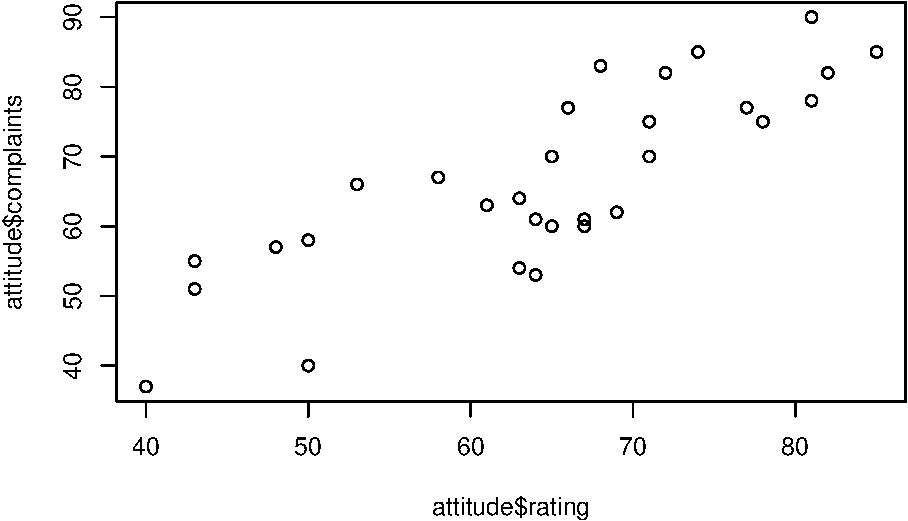
\includegraphics{main_files/figure-latex/unnamed-chunk-2-1.pdf}
\caption{A caption}
\end{figure}

\newpage

\hypertarget{references}{%
\section*{References}\label{references}}
\addcontentsline{toc}{section}{References}

\hypertarget{refs}{}
\leavevmode\hypertarget{ref-bae2014invariance}{}%
Bae, Kyounghun, Albert S Kyle, Eun Jung Lee, and Anna A Obizhaeva. 2014.
``An Invariance Relationship in the Number of Buy-Sell Switching
Points.'' Working Paper, University of Maryland.

\end{document}
